\documentclass{beamer}
\usepackage[utf8]{inputenc}

\usepackage{semantic}
\usepackage{graphicx}
\usepackage{booktabs}
%\usepackage{todonotes}
\usepackage[absolute,overlay]{textpos}
\usepackage{tikz}

\mode<presentation> {
\usetheme{boxes} % When headline is wanted use Dresden theme instead
\usecolortheme{seagull}
\setbeamertemplate{footline}[page number]
\setbeamertemplate{navigation symbols}{}
}


% APL LaTeX declarations, based on work by A.Hohti/O.Kanerva
% University of Helsinki April 6 1987
%
% Written Oct. 3rd 2006 by Markus Triska (triska@gmx.at)
% Public domain code.

\font\apl=cmapl10 at 9pt      % The APL font of typewriter type

% from:
%		apldef.tex
%
% 2-letter control sequences for using cmapl10.
%===============================================================
%
\def\RO{{\apl\char'014}}               % rho
\def\IO{{\apl\char'015}}               % iota
\def\BX{\hskip0pt\lower.1ex\hbox{\apl\char'001}}               % quad box (window etc.)
\def\CE{{\apl\char'035}}               % ceiling
\def\FL{{\apl\char'034}}               % floor
\def\DE{{\apl\char'031}}               % decode
\def\EN{{\apl\char'030}}               % encode
\def\DL{{\apl\char'002}}               % del
\def\LD{{\apl\char'003}}               % delta
\def\NT{{\apl\char'026}}               % not
\def\LO{{\apl\char'017}}               % circle
\def\GO{{\apl\char'036}}               % arrow right
\def\OR{{\apl\char'010}}               % logical or
\def\DM{{\apl\char'011}}               % diamond
\def\LE{{\apl\char'012}}               % less than or equal
\def\GE{{\apl\char'013}}               % greater than or equal
\def\AB{{\apl\char'174}}               % stile
\def\LB{{\apl\char'173}}               % left brace
\def\RB{{\apl\char'175}}               % right brace
\def\DA{{\apl\char'037}}               % arrow down
\def\UA{{\apl\char'136}}               % arrow up
\def\EP{{\apl\char'006}}               % epsilon
\def\NE{{\apl\char'027}}               % not equal
\def\BL{{\apl\char'134}}               % backslash
\def\RU{{\apl\char'022}}               % right U
\def\LU{{\apl\char'023}}               % left U
\def\DU{{\apl\char'021}}               % down U
\def\UU{{\apl\char'020}}               % up U
\def\LK{{\apl\char'033}}               % right tack
\def\RK{{\apl\char'032}}               % left tack
\def\US{{\apl\char'024}}               % underscore
\def\NG{{\apl\char'025}}               % high minus
\def\DD{{\apl\char'007}}               % dieresis
\def\AM{{\apl\char'004}}               % alpha
\def\OM{{\apl\char'005}}               % omega
\def\SO{\leavevmode\raise.3ex\hbox{{\apl\char'016}}} % small circle
%
% This macro is used for overstriking two characters
\newskip\charwidth
\def\overstrike#1#2{\setbox1=\hbox{#1}\charwidth=\wd1
           #1\hskip-\charwidth#2}
%
\def\TR{\overstrike{\LO}{\BL}}                              % transpose
\def\RV{\overstrike{\LO}{\AB}}                              % reverse
\def\CR{\overstrike{\leavevmode\raise.1ex\hbox{\hskip0.361pt -}}{\LO}}
                                                   % column reverse
\def\GD{\overstrike{\DL}{\AB}}                              % grade down
\def\GU{\overstrike{\LD}{\AB}}                              % grade up
\def\FM{\overstrike{\leavevmode\raise.1ex\hbox{{\apl\char'016}}}{\EN}} % format
\def\XQ{\overstrike{\leavevmode\raise.1ex\hbox{{\apl\char'016}}}{\DE}} % execute
\def\SS{\overstrike{\RU}{\US}}                              % subset
\def\CO{\overstrike{\LU}{\US}}                              % contains
\def\CB{\overstrike{\BL}{-}}                                % column backslash
\def\CS{\overstrike{/}{-}}                                  % column slash
\def\IB{\overstrike{\EN}{\DE}}                              % I-beam
\def\DQ{\overstrike{{\apl\char'045}}{\BX}}                  % divide quad
\def\QQ{\overstrike{{\apl '}}{\BX}}                         % quote quad
\def\PD{\overstrike{\DL}{\NT}}                              % protected del
\def\NR{\overstrike{\OR}{\NT}}                              % nor
\def\NN{\overstrike{{\apl\char'046}}{\NT}}                  % nand
\def\LG{\overstrike{{\apl *}}{\LO}}                         % logarithm
\def\PO{\overstrike{\DD}{\apl *}}
% underscored letters
\def\ZA{\overstrike{{\apl A}}{\US}}
\def\ZB{\overstrike{{\apl B}}{\US}}
\def\ZC{\overstrike{{\apl C}}{\US}}
\def\ZD{\overstrike{{\apl D}}{\US}}
\def\ZE{\overstrike{{\apl E}}{\US}}
\def\ZF{\overstrike{{\apl F}}{\US}}
\def\ZG{\overstrike{{\apl G}}{\US}}
\def\ZH{\overstrike{{\apl H}}{\US}}
\def\ZI{\overstrike{{\apl I}}{\US}}
\def\ZJ{\overstrike{{\apl J}}{\US}}
\def\ZK{\overstrike{{\apl K}}{\US}}
\def\ZL{\overstrike{{\apl L}}{\US}}
\def\ZM{\overstrike{{\apl M}}{\US}}
\def\ZN{\overstrike{{\apl N}}{\US}}
\def\ZO{\overstrike{{\apl O}}{\US}}
\def\ZP{\overstrike{{\apl P}}{\US}}
\def\ZQ{\overstrike{{\apl Q}}{\US}}
\def\ZR{\overstrike{{\apl R}}{\US}}
\def\ZS{\overstrike{{\apl S}}{\US}}
\def\ZT{\overstrike{{\apl T}}{\US}}
\def\ZU{\overstrike{{\apl U}}{\US}}
\def\ZV{\overstrike{{\apl V}}{\US}}
\def\ZX{\overstrike{{\apl X}}{\US}}
\def\ZY{\overstrike{{\apl Y}}{\US}}
\def\ZW{\overstrike{{\apl W}}{\US}}
\def\ZZ{\overstrike{{\apl Z}}{\US}}

% unicode declarations

% first row
\DeclareUnicodeCharacter{22C4}{\DM} % diamond
\DeclareUnicodeCharacter{223C}{\NT} % not
\DeclareUnicodeCharacter{00A8}{\DD} % dieresis
\DeclareUnicodeCharacter{2336}{\IB} % I-Beam
\DeclareUnicodeCharacter{00AF}{\NG} % high minus
\DeclareUnicodeCharacter{236B}{\PD} % protected del
\DeclareUnicodeCharacter{2352}{\GD} % grade down
\DeclareUnicodeCharacter{2264}{\LE} % less than or equal
\DeclareUnicodeCharacter{234B}{\GU} % grade up
\DeclareUnicodeCharacter{233D}{\RV} % reverse
\DeclareUnicodeCharacter{2265}{\GE} % greater or equal
\DeclareUnicodeCharacter{2349}{\TR} % transpose
\DeclareUnicodeCharacter{2296}{\CR} % column reverse
\DeclareUnicodeCharacter{2260}{\NE} % not equal
\DeclareUnicodeCharacter{235F}{\LG} % logarithm
\DeclareUnicodeCharacter{2228}{\OR} % logical or
\DeclareUnicodeCharacter{2371}{\NR} % nor
\DeclareUnicodeCharacter{2227}{{\apl\char'046}} % and
\DeclareUnicodeCharacter{2372}{\NN} % nand
\DeclareUnicodeCharacter{00D7}{{\apl\char'043}} % times
\DeclareUnicodeCharacter{00F7}{{\apl\char'045}} % division
\DeclareUnicodeCharacter{2339}{\DQ} % divide quad / matrix division
% second row
\DeclareUnicodeCharacter{2375}{\OM} % omega
\DeclareUnicodeCharacter{2208}{\EP} % epsilon
\DeclareUnicodeCharacter{2377}{\overstrike{\EP}{\US}} % underscore epsilon
\DeclareUnicodeCharacter{2374}{\RO} % rho
\DeclareUnicodeCharacter{2191}{\UA} % up arrow
\DeclareUnicodeCharacter{2193}{\DA} % down arrow
\DeclareUnicodeCharacter{2373}{\IO} % iota
\DeclareUnicodeCharacter{2378}{\overstrike{\IO}{\US}} % underscore iota
\DeclareUnicodeCharacter{25CB}{\LO} % circle
\DeclareUnicodeCharacter{2365}{\overstrike{\DD}{\LO}} % circle dieresis
\DeclareUnicodeCharacter{22C6}{{\apl *}} % exponentiation
\DeclareUnicodeCharacter{235F}{\LG} % logarithm
\DeclareUnicodeCharacter{2190}{{\apl\char'137}} % arrow left
\DeclareUnicodeCharacter{2192}{\GO} % arrow right
\DeclareUnicodeCharacter{2340}{\CB} % column backslash
\DeclareUnicodeCharacter{2359}{\overstrike{\US}{\LD}} % delta underscore
% third row
\DeclareUnicodeCharacter{237A}{\AM} % alpha
\DeclareUnicodeCharacter{2296}{\CR} % column reverse
\DeclareUnicodeCharacter{2308}{\CE} % ceiling
\DeclareUnicodeCharacter{230A}{\FL} % floor
\DeclareUnicodeCharacter{2261}{$\equiv$}
\DeclareUnicodeCharacter{2207}{$\nabla$}
\DeclareUnicodeCharacter{2352}{\GD} % grade down
\DeclareUnicodeCharacter{2206}{\LD} % delta
\DeclareUnicodeCharacter{2218}{\SO} % jot
\DeclareUnicodeCharacter{2364}{\"\relax\hskip-5.8pt\SO} % jot dieresis
\DeclareUnicodeCharacter{233C}{\overstrike{\BX}{\LO}} % quad circle
\DeclareUnicodeCharacter{2395}{\BX} % quad
\DeclareUnicodeCharacter{235E}{\QQ} % quote quad
\DeclareUnicodeCharacter{22A2}{\LK} % right tack
\DeclareUnicodeCharacter{2342}{\overstrike{\BX}{\BL}} % quad backslash
\DeclareUnicodeCharacter{22A3}{\RK} % left tack
\DeclareUnicodeCharacter{233C}{\overstrike{\BX}{\LO}} % quad circle
\DeclareUnicodeCharacter{2282}{\RU} % right u
\DeclareUnicodeCharacter{2283}{\LU} % left u
\DeclareUnicodeCharacter{2229}{\DU} % down u
\DeclareUnicodeCharacter{235D}{{\apl\char'042}} % comment sign
\DeclareUnicodeCharacter{222A}{\UU} % up u
\DeclareUnicodeCharacter{22A5}{\DE} % decode
\DeclareUnicodeCharacter{234E}{\XQ} % execute
\DeclareUnicodeCharacter{22A4}{\EN} % encode
\DeclareUnicodeCharacter{2355}{\FM} % format
\DeclareUnicodeCharacter{2223}{\AB} % stile
\DeclareUnicodeCharacter{233F}{\CS} % column slash
\DeclareUnicodeCharacter{2212}{-}   % minus
\DeclareUnicodeCharacter{2262}{$\not\equiv$}
\DeclareUnicodeCharacter{220A}{\EP} % small contains, alternative for member
\DeclareUnicodeCharacter{2217}{{\apl *}} % asterisk, alternative for star
\DeclareUnicodeCharacter{03BA}{$\kappa$}
\DeclareUnicodeCharacter{2363}{\overstrike{\DD}{{\apl *}}}

\newcommand{\kw}[1]{\texttt{#1}}
\newcommand{\A}[2]{[#1]^{#2}}
\newcommand{\V}[2]{\langle#1\rangle^{#2}}
\renewcommand{\S}[2]{\textrm{S}_{#1}(#2)}
\newcommand{\SV}[2]{\textrm{SV}_{#1}(#2)}
\newcommand{\id}[1]{\textit{#1}}

\newcommand{\IOt}{\texttt{\IO}}
\newcommand{\DDt}{\texttt{\DD}}
\newcommand{\ROt}{\texttt{\RO}}
\newcommand{\UAt}{\texttt{\UA}}
\newcommand{\DAt}{\texttt{\DA}}
\newcommand{\LUt}{\texttt{\LU}}
\newcommand{\TRt}{\texttt{\TR}}
\newcommand{\RVt}{\texttt{\RV}}
\newcommand{\POt}{\texttt{\PO}}
\newcommand{\FMt}{\texttt{\FM}}


%----------------------------------------------------------------------------------------
%	TITLE PAGE
%----------------------------------------------------------------------------------------

\title[FCL] % bottom of every slide
  {FCL: A low-level functional GPU language} % title page

\subtitle{(Very much work in progess)}

\author{\footnotesize{Martin Dybdal} \\ \footnotesize{\texttt{dybber@dybber.dk}}}

\institute {
HIPERFIT \\
DIKU \\
University of Copenhagen
}

\date{\footnotesize{HIPERFIT workshop, 4 March 2016}}

% \title[Group Theory]{A longer title of the talk concerning Group Theory}
% \author[short name]{My full name}
% \institute[My Inst.]{Full Institut Name}
% % logo of my university

\date[4 March 2016]{4 March 2016}

\begin{document}

{
\setbeamertemplate{headline}{}
\begin{frame}
  \titlepage

  \note{I started thinking during master thesis, ~ 3 years
    ago. decided to start top down.}
\end{frame}
}

%----------------------------------------------------------------------------------------
%	TABLE OF CONTENTS
%----------------------------------------------------------------------------------------

% \begin{frame}
% \frametitle{Overview}
% \tableofcontents
% \end{frame}

%----------------------------------------------------------------------------------------
%	CONTENT
%----------------------------------------------------------------------------------------


\section{Overview}

\begin{frame}[fragile]
\frametitle{Previously: APL $->$ TAIL}
{\footnotesize
\begin{verbatim}
pi ← { 
 x ← ?⍵⍴0
 y ← ?⍵⍴0
 dists ← (x*2) + y*2
 4×(+/1>dists)÷⍵
}
pi 1000000
    3.142668
\end{verbatim}
\pause
\vspace{-2mm}
$\quad\Downarrow$
\vspace{-2mm}
% muld(4.0,
%  divd(i2d(
%    reduce(addi,0,
%      each(b2i,
%        each(fn v7:[double]0 => gtd(1.0,v7),
%          each(fn v6:[double]0 => powd(v6,divd(1.0,2.0)),
%            reduce(addd,0.0,
%              each(fn v3:[double]0 => powd(v3,2.0),
%                each(fn v2:[bool]0 => roll(b2i(v2)),
%                     reshape([1000000,2],[ff]))))))))),
%       1000000.0))
\begin{verbatim}
let v3:[double]1 = 
  each(fn v2:[int]0 => roll(v2), reshape([1000000],[0])) in
let v5:[double]1 =
  each(fn v4:[int]0 => roll(v4), reshape([1000000],[0])) in
let v11:[double]1 = 
  each(fn v10:[double]0 => powd(v10,divd(1.0,2.0)),
       zipWith(addd, each(fn v7:[double]0 => powd(v7,2.0),v3),
                     each(fn v6:[double]0 => powd(v6,2.0),v5))) in
muld(4.0, divd(i2d(reduce(addi,0,
                     each(b2i,
                       each(fn v12:[double]0 => gtd(1.0,v12),
                            v11)))),
               1000000.0))
\end{verbatim}
}

\begin{textblock*}{64mm}(0.50\textwidth,0.43\textheight)
\only<2->{
\begin{block}{\vspace*{-3ex}}
Note: \texttt{each} is just \texttt{map} in APL lingo
\end{block}
}
\end{textblock*}

\end{frame}

\begin{frame}[fragile]
\frametitle{APL $->$ TAIL $->$ ?}
\begin{center}
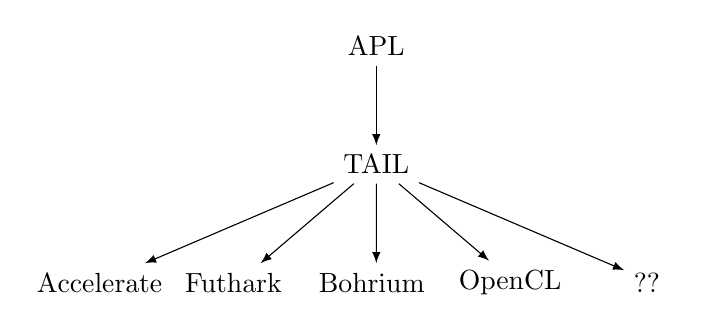
\begin{tikzpicture}[edge from parent/.style={draw,-latex},
                    sibling distance=5em,
                    every node/.style = {shape=rectangle,
                    align=center}]
  \node {APL}
    child { node {TAIL}
      child { node {Accelerate} }
      child { node { Futhark } }
      child { node { Bohrium } }
      child { node { OpenCL } }
      child { node { ?? } }
    };
\end{tikzpicture}
\end{center}
\end{frame}


\begin{frame}
\frametitle{Outline}

~APL \\
$\quad\Downarrow$ \\
~TAIL \\
$\quad\Downarrow$\\
~~\ldots \\
$\quad\Downarrow$ \\
\fbox{FCL: a low-level GPU language} \\
$\quad\Downarrow$ \\
OpenCL/CUDA
\end{frame}

\begin{frame}
\frametitle{Obsidian overview}
\begin{itemize}
\item GPU language embedded in Haskell
\item Two-layer design with Haskell as meta-language
\item Hierarchy of array types
\item Loops are always unrolled
\item Some array sizes must be known statically
\end{itemize}
\end{frame}

\begin{frame}[fragile]
  \frametitle{Obsidian example: reduction}

\begin{verbatim}
simpleReduce :: Data a 
             => (a -> a -> a)
             -> SPull a
             -> Program Block (SPush Block a)
simpleReduce f arr =
  if len arr == 1
  then return (push arr)
  else do let (a1,a2) = halve arr
          arr' <- computePull (zipWith f a1 a2)
          simpleReduce f arr'
\end{verbatim}
\pause
\begin{itemize}
\item Specifies reduction in a single block
\item Generates an unrolled loop
\end{itemize}
\end{frame}

\begin{frame}[fragile]
  \frametitle{Obsidian example: reduction}

\begin{verbatim}
simpleReduce :: Data a 
             => (a -> a -> a)
             -> SPull a
             -> Program Block (SPush Block a)

red :: Data a
    => (a -> a -> a)
    -> DPull (SPull a)
    -> DPush Grid a
red f arr = liftGridMap (execBlock . simpleReduce f) arr

addReduce  :: DPull EInt32 -> DPush Grid EInt32
addReduce = red (+) . splitUp 512
\end{verbatim}
\pause
\begin{itemize}
\item \texttt{red} lifts reduction to grid-level
\item \texttt{splitUp} creates a nested array of arrays
\item To do a full reduction, the kernel should be applied repeatedly.
\end{itemize}
\end{frame}

\begin{frame}[fragile]
  \frametitle{Obsidian summary}

\begin{itemize}
\item EDSL
\item Generates \textit{individual} CUDA kernels
\item Fusion-by-default, but user controlled
\item Meta-programming
\item Program GPU hierarchy in uniform style
\end{itemize}
\end{frame}



\begin{frame}
\frametitle{Goals of FCL}
\begin{itemize}
\item Close to the metal
\item Built in fusion, but user-controlled
\item Predictability, no black box
\item Ability to optimize
\item Expressive enough for all necessary APL primitives
\item A GPU language for algorithms researchers?
\item Starting point: ``Unembedded Obsidian''
\end{itemize}
\end{frame}

\begin{frame}[fragile]
\frametitle{FCL reverse}

\begin{verbatim}
sig reverse : [a] -> [a]
fun reverse arr =
  let n = length arr
  in generate n (fn i => index arr (n - i - 1))
\end{verbatim}

\pause
\begin{verbatim}
sig distributeReverse : int -> [a] -> [a]
fun distributeReverse splitSize arr =
  splitUp splitSize arr
   |> map (fn subarr => force (reverse subarr))
   |> reverse
   |> concat splitSize
\end{verbatim}

\pause
\begin{verbatim}
sig reverseKernel : [int] -> [int]
kernel reverseKernel arr = distributeReverse 512 arr
\end{verbatim}
\end{frame}


\begin{frame}[fragile]
  \frametitle{OpenCL}
{\tiny
  \begin{verbatim}
__kernel void reverseGridKernel(__local uchar* sbase,__global int* arrInput_0,
                                int lenInput_1, __global int* arrOutput_3) {
  int n_2 = ((lenInput_1 + get_local_size(0)) - 1) / get_local_size(0);
  int ub_5 = n_2;
  int id17 = ub_5 / get_num_groups(0);
  __local int* arr_7 = (__local int*) (sbase + 0);
  for (int id16 = 0; id16 < id17; id16++) {
    int i_4 = (get_group_id(0) * id17) + id16;
    for (int id12 = 0; id12 < 1; id12++) {
      int i_8 = (id12 * get_local_size(0)) + get_local_id(0);
      arr_7[i_8] = arrInput_0 [((((n_2-i_4)-1)*get_local_size(0)) + ((get_local_size(0)-i_8)-1))];
    }
    barrier(CLK_LOCAL_MEM_FENCE);
    for (int id14 = 0; id14 < 1; id14++) {
      int i_10 = (id14 * get_local_size(0)) + get_local_id(0);
      arrOutput_3[((i_4 * get_local_size(0)) + i_10)] = arr_7 [i_10];
    }
    barrier(CLK_LOCAL_MEM_FENCE);
  }
  if (get_group_id(0) < (ub_5 % get_num_groups(0))) {
    int i_4 = (get_num_groups(0) * id17) + get_group_id(0);
    for (int id12 = 0; id12 < 1; id12++) {
      int i_8 = (id12 * get_local_size(0)) + get_local_id(0);
      arr_7[i_8] = arrInput_0 [((((n_2-i_4)-1)*get_local_size(0)) + ((get_local_size(0)-i_8)-1))];
    }
    barrier(CLK_LOCAL_MEM_FENCE);
    for (int id14 = 0; id14 < 1; id14++) {
      int i_10 = (id14 * get_local_size(0)) + get_local_id(0);
      arrOutput_3[((i_4 * get_local_size(0)) + i_10)] = arr_7 [i_10];
    }
    barrier(CLK_LOCAL_MEM_FENCE);
  }
}
\end{verbatim}
}
\end{frame}

\begin{frame}[fragile]
\frametitle{\texttt{concat} and \texttt{assemble}}

Concatenation is a derived form:
\begin{verbatim}
  sig concat : int -> [[a]] -> [a]
  fun concat n arr =
    assemble n (fn sh => (fst sh * n) + snd sh) arr
\end{verbatim}
\vspace{5mm}
\pause
Using a more general construct ``assemble'':
\begin{verbatim}
  assemble : int -> ((int, int) -> int) -> [[a]] -> [a]
\end{verbatim}

\end{frame}


\begin{frame}[fragile]
\frametitle{Transpose}
{\footnotesize

\begin{verbatim}
sig transpose : int -> int -> [a] -> [a]
fun transpose rows cols elems =
  generate (rows * cols)
           (fn n =>
              let i = n / rows in
              let j = n % rows
              in index elems (j * rows + i))
\end{verbatim}

\pause
\begin{verbatim}
splitGrid : int -> int -> int -> [a] -> [[a]]
concatGrid : int -> int -> [[a]] -> [a]
\end{verbatim}

\pause
\begin{verbatim}
sig transposeChunked : int -> int -> int -> [int] -> [int]
kernel transposeChunked splitSize rows cols elems =
  splitGrid splitSize rows cols elems
    |> map (transpose splitSize splitSize)
    |> map (fn arr => force arr)  -- force into shared memory
    |> transpose (rows / splitSize) (cols / splitSize)
    |> concatGrid splitSize (cols / splitSize)
\end{verbatim}
}
\end{frame}

\begin{frame}[fragile]
  \frametitle{Reduction}
\begin{verbatim}
sig reduceBlock : (a -> a -> a) -> [a] -> [a]
fun reduceBlock f arr =
  let cond = fn arr => 1 <> length arr in
  let step = fn arr => let x = halve arr
                       in zipWith f (fst x) (snd x)
  in while cond step (step arr)
\end{verbatim}
\pause
\begin{verbatim}
sig reducePart : (a -> a -> a) -> [a] -> [a]
fun reducePart f arr =
  splitUp 512 arr
   |> map (reduceBlock f)
   |> concat 1
\end{verbatim}
\end{frame}

\begin{frame}
  \frametitle{Future work on FCL}
  \begin{itemize}
  \item GPU-hierarchy in types
  \item Loop unrolling annotations
  \item Host-code generation
  \item Larger examples
  \item (Shapes and multi-dimensional arrays)
  \end{itemize}
\end{frame}


\begin{frame}
  \frametitle{Future work on TAIL and FCL}
  \begin{itemize}
  \item FCL as backend for TAIL
  \item TAIL annotations for GPU vs. CPU execution
  \item Multiple devices (another level in the hierarchy?)
  \item Ability to inline FCL within APL program
  \item Integration with real APL interpreter (Dyalog)
  \end{itemize}
\end{frame}

\begin{frame}
\frametitle{References}
\footnotesize{
\begin{thebibliography}{99} % Beamer does not support BibTeX so references must be inserted manually as below
\bibitem{p1} Compiling a Subset of APL Into a Typed Intermediate Language.
\newblock Martin Elsman and Martin Dybdal, 2014
\newblock \emph{ARRAY'14}

\bibitem{p1} Obsidian: A domain specific embedded language for parallel programming of graphics processor
\newblock Joel Svensson, Mary Sheeran, Koen Claessen, 2011
\newblock \emph{IFL'11}

\end{thebibliography}
}
\end{frame}

\begin{frame}
\Huge{\centerline{Questions?}}
\end{frame}


%----------------------------------------------------------------------------------------
%	BEAMER EXAMPLES of column layouts and tables
%----------------------------------------------------------------------------------------

% \begin{frame}
% \frametitle{Multiple Columns}
% \begin{columns}[c] % The "c" option specifies centered vertical alignment while the "t" option is used for top vertical alignment

% \column{.45\textwidth} % Left column and width

% \column{.5\textwidth} % Right column and width

% \end{columns}
% \end{frame}

% \begin{frame}
% \frametitle{Table}
% \begin{table}
% \begin{tabular}{l l l}
% \toprule
% \textbf{Treatments} & \textbf{Response 1} & \textbf{Response 2}\\
% \midrule
% Treatment 1 & 0.0003262 & 0.562 \\
% Treatment 2 & 0.0015681 & 0.910 \\
% Treatment 3 & 0.0009271 & 0.296 \\
% \bottomrule
% \end{tabular}
% \caption{Table caption}
% \end{table}
% \end{frame}

\end{document}